% 90-23(90쪽) — 가로 16 cm, 세로 10 cm 인 직사각형 모양의 종이에서 네 귀퉁이의 정사각형을 잘라 내는 그림(접는 선은 점선 · 남는 부분 색칠). 스캔 화질이 낮아 TikZ 로 다시 그림.
% 원문에 있는 것만 옮긴다: 직사각형 · 네 귀퉁이의 정사각형 · 접는 점선 · 치수 16 cm, 10 cm. 잘라 내는 정사각형의 한 변은 원문 그림의 크기 그대로 그려 답(부피가 최대인 한 변의 길이)을 읽을 수 없게 한다.
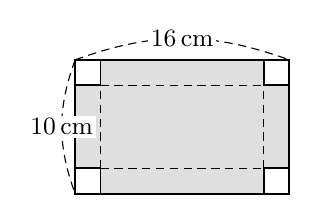
\begin{tikzpicture}[x=0.17cm, y=0.17cm, line width=0.6pt]
  \fill[gray!25] (1.9,0) rectangle (14.1,10);
  \fill[gray!25] (0,1.9) rectangle (16,8.1);
  \draw (0,0) rectangle (16,10);
  % 네 귀퉁이에서 잘라 내는 정사각형
  \draw (1.9,0) -- (1.9,1.9) -- (0,1.9);
  \draw (14.1,0) -- (14.1,1.9) -- (16,1.9);
  \draw (1.9,10) -- (1.9,8.1) -- (0,8.1);
  \draw (14.1,10) -- (14.1,8.1) -- (16,8.1);
  % 접는 선
  \draw[densely dashed, line width=0.4pt] (1.9,1.9) -- (14.1,1.9);
  \draw[densely dashed, line width=0.4pt] (1.9,8.1) -- (14.1,8.1);
  \draw[densely dashed, line width=0.4pt] (1.9,1.9) -- (1.9,8.1);
  \draw[densely dashed, line width=0.4pt] (14.1,1.9) -- (14.1,8.1);
  % 치수
  \draw[densely dashed, line width=0.4pt] (0,10) to[bend left=20] node[midway, fill=white, inner sep=1pt, font=\small] {$16\,\mathrm{cm}$} (16,10);
  \draw[densely dashed, line width=0.4pt] (0,10) to[bend right=20] node[midway, fill=white, inner sep=1pt, font=\small] {$10\,\mathrm{cm}$} (0,0);
\end{tikzpicture}
